\documentclass[11pt, a4paper]{report}
\usepackage[utf8]{inputenc}
\usepackage{pgfplots}

\usepackage[top=2cm, bottom=2.3cm, left=2cm, right=2cm]{geometry}

\title{Graficos das geracoes do NSGA2}
\author{Douglas Nunes de Oliveira}
\date{November 2021}


\begin{document}
    \begin{center}
        \textbf{Utilizando o NSGA2 para o problema de Schaffer modificado.}
        
        \textbf{Gráficos do espaço dos objetivos nas gerações ``1, 10, 50, 100 e 1000''}
        
        
    \end{center}
    

    \begin{center}
    \textbf{Geração 1}
\end{center}

\begin{figure}[h]
    \centering
    \label{fig:geracao01}
    
    \begin{tabular}{rl}
        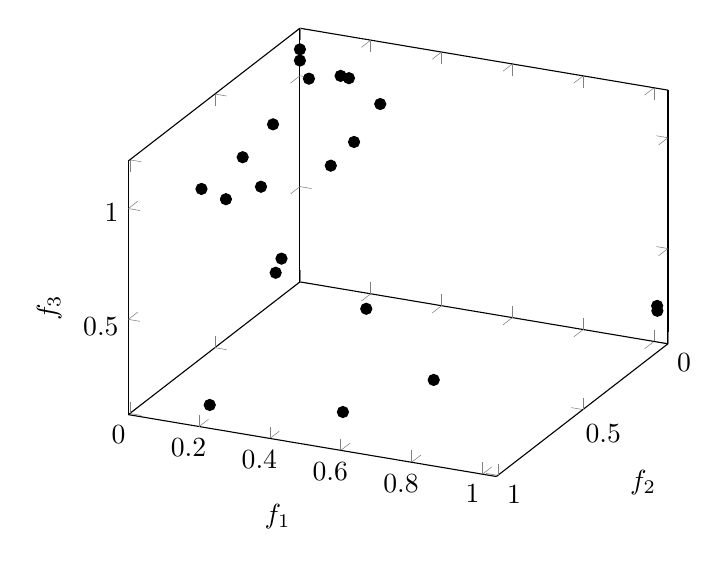
\begin{tikzpicture}[scale=1.0]
        	\begin{axis}[xlabel=$f_2$, ylabel=$f_1$, zlabel=$f_3$, view/h=115]
    			
    			\addplot3[only marks] coordinates {
            		(0.898985, 0.553341, 0.165563) (1.008660, 0.229953, 0.175532) (0.062171, 1.039330, 0.255872) (0.000000, 0.000000, 1.068948) (0.000000, 0.000000, 1.119406) (0.813499, 0.578235, 0.587300) (0.055647, 1.035543, 0.273132) (0.709822, 0.718883, 0.242456) (0.776314, 0.304513, 0.654200) (0.586016, 0.072568, 0.810780) (0.694715, 0.281731, 0.663309) (0.263698, 0.279511, 0.933176) (0.523794, 0.141747, 0.848635) (0.095871, 0.071497, 1.063344) (0.378926, 0.269237, 0.891967) (0.625020, 0.022316, 0.866778) (0.022923, 0.149424, 1.043225) (0.435767, 0.047729, 0.904337) (0.295924, 0.066268, 0.974661) (0.023673, 0.126287, 1.047775) (0.047674, 0.249717, 0.968201) 


        		};
        	\end{axis}
	    \end{tikzpicture}
	    &
	    \begin{tikzpicture}[scale=1.0]
        	\begin{axis}[xlabel=$f_2$, ylabel=$f_1$, zlabel=$f_3$, view={45}{0}]
    			
    			\addplot3[only marks] coordinates {
            		(0.198659,1.402927,0.030436)(0.243016,1.009920,0.490406)(0.965942,0.316067,0.944104)(0.926777,1.057248,0.066572)(0.755361,1.454336,0.018711)(1.099215,0.001117,0.701296)(0.930406,0.386454,0.145874)(0.363359,0.141019,1.073644)(0.005555,0.002258,1.133576)(1.244191,0.475865,0.000000)(0.055722,1.206260,0.087339)(0.122153,0.960673,0.791197)(1.197703,0.000000,0.012183)(0.338440,0.645361,1.002919)(1.231961,0.176431,0.126477)(0.842002,1.466963,0.128832)(1.400163,0.069214,0.140365)(0.050612,0.297072,1.183874)(0.177113,0.032273,1.369730)(0.096804,0.169118,1.443461)(1.185475,0.441860,0.309690) 

        		};
        	\end{axis}
	    \end{tikzpicture}
	\end{tabular}
    
\end{figure}


    \hrulefill
    \begin{center}
    \textbf{Geração 10}
\end{center}

\begin{figure}[h]
    \centering
    \label{fig:geracaoXX}
    
    \begin{tikzpicture}[scale=1.4]
        \begin{axis}[enlargelimits=false]
            \addplot [] coordinates {
                (0.000000,4.000000) (0.010000,3.610000) (0.040000,3.240000) (0.090000,2.890000) (0.160000,2.560000) (0.250000,2.250000) (0.360000,1.960000) (0.490000,1.690000) (0.640000,1.440000) (0.810000,1.210000) (1.000000,1.000000) (1.210000,0.810000) (1.440000,0.640000) (1.690000,0.490000) (1.960000,0.360000) (2.250000,0.250000) (2.560000,0.160000) (2.890000,0.090000) (3.240000,0.040000) (3.610000,0.010000) (4.000000,0.000000) 
            };
            
            \addplot [only marks] coordinates {
                (9.765582,16.939883)(9.924204,17.003386)(10.091199,17.110039)(10.211898,17.205926)(10.337007,17.555696)(12.514860,17.518859)(13.126414,18.337417)(17.804570,20.690929)(70.410450,56.563290)(71.896435,90.028819)(72.099991,90.135653)(72.732258,90.743713)(72.980565,91.249132)(73.640637,91.289447)(73.857270,91.995217)(75.358388,92.246202)(75.811555,94.296171)(76.248114,94.129894)(76.362091,94.174254)(76.250749,94.632550) 
            };
        \end{axis}
    \end{tikzpicture}
\end{figure}

    \newpage

    \begin{center}
    \textbf{Geração 50}
\end{center}

\begin{figure}[h]
    \centering
    \label{fig:geracaoXX}
    
    \begin{tikzpicture}[scale=1.4]
        \begin{axis}[enlargelimits=false]
            \addplot [] coordinates {
                (0.000000,4.000000) (0.010000,3.610000) (0.040000,3.240000) (0.090000,2.890000) (0.160000,2.560000) (0.250000,2.250000) (0.360000,1.960000) (0.490000,1.690000) (0.640000,1.440000) (0.810000,1.210000) (1.000000,1.000000) (1.210000,0.810000) (1.440000,0.640000) (1.690000,0.490000) (1.960000,0.360000) (2.250000,0.250000) (2.560000,0.160000) (2.890000,0.090000) (3.240000,0.040000) (3.610000,0.010000) (4.000000,0.000000) 
            };
            
            \addplot [only marks] coordinates {
                (7.079039,9.893604)(6.998996,10.667901)(7.153247,10.267265)(7.675170,10.023482)(7.176644,10.167450)(7.684816,10.057420)(7.337534,10.589789)(7.258915,11.093974)(7.387049,10.466614)(7.385134,10.873843)(7.421006,10.594347)(7.413217,11.198653)(7.536725,10.792519)(7.722630,10.658570)(7.437473,10.984634)(7.596418,10.718251)(7.577853,11.008782)(7.721938,10.867479)(8.215063,10.807069)(8.124915,10.913137)
            };
        \end{axis}
    \end{tikzpicture}
\end{figure}
    \hrulefill
    \begin{center}
    \textbf{Geração 100}
\end{center}

\begin{figure}[h]
    \centering
    \label{fig:geracao01}
    
    \begin{tabular}{rl}
        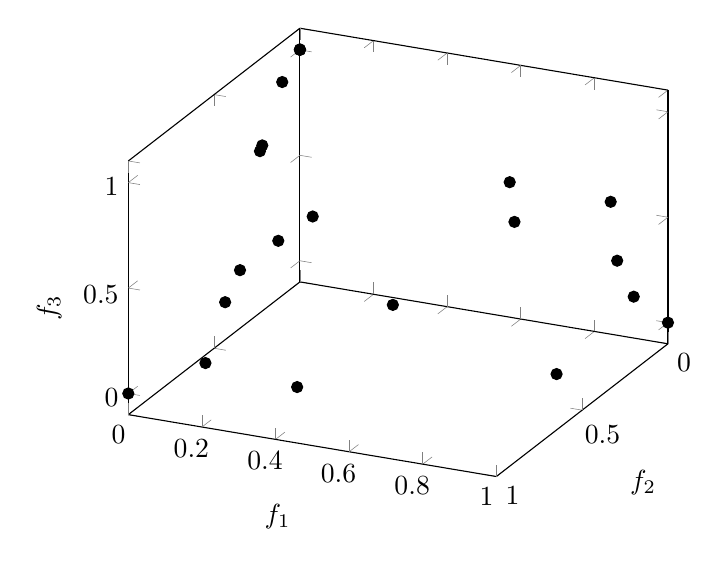
\begin{tikzpicture}[scale=1.0]
        	\begin{axis}[xlabel=$f_2$, ylabel=$f_1$, zlabel=$f_3$, view/h=115]
    			\addplot3[only marks] coordinates {
            		(1.000000, 0.000000, 0.000000) (0.000000, 1.000000, 0.000000) (0.000000, 0.000000, 1.000000) (0.000000, 0.000000, 1.000000) (0.000000, 0.000000, 1.002366) (0.705447, 0.581417, 0.405378) (0.320760, 0.732482, 0.601146) (0.219298, 0.672219, 0.707855) (0.631412, 0.329124, 0.703873) (0.906018, 0.414925, 0.093147) (0.818324, 0.218773, 0.534681) (0.490308, 0.120026, 0.863611) (0.883003, 0.208553, 0.420490) (0.134857, 0.924880, 0.356595) (0.007624, 0.847914, 0.533176) (0.194546, 0.042607, 0.982411) (0.965028, 0.193231, 0.179025) (0.435372, 0.900348, 0.001011) (0.724088, 0.278846, 0.632154) (0.468641, 0.116210, 0.876071) (0.136309, 0.970537, 0.200331) 

        		};
        	\end{axis}
	    \end{tikzpicture}
	    &
	    \begin{tikzpicture}[scale=1.0]
        	\begin{axis}[xlabel=$f_2$, ylabel=$f_1$, zlabel=$f_3$, view={45}{0}]
    			\addplot3[only marks] coordinates {
            		(1.000406,0.000000,0.000000)(0.000000,1.000821,0.000000)(0.000000,0.000000,1.000410)(0.000000,0.000000,1.000513)(0.000000,0.000000,1.008846)(0.428855,0.738966,0.536111)(0.376896,0.857096,0.353981)(0.060711,0.545878,0.837624)(0.577614,0.780391,0.241495)(0.648720,0.240773,0.740718)(0.500330,0.869753,0.178641)(0.771673,0.451443,0.449195)(0.871780,0.307549,0.387998)(0.975467,0.019472,0.228255)(0.027904,0.484476,0.875860)(0.231686,0.510675,0.829175)(0.490248,0.825942,0.289970)(0.828461,0.410978,0.383852)(0.212737,0.088363,0.975027)(0.730887,0.335500,0.608352)(0.483225,0.876988,0.015638) 

        		};
        	\end{axis}
	    \end{tikzpicture}
	\end{tabular}
    
\end{figure}


    
    \newpage
    \begin{center}
    \textbf{Geração 1000}
\end{center}

\begin{figure}[h]
    \centering
    \label{fig:geracaoXX}
    
    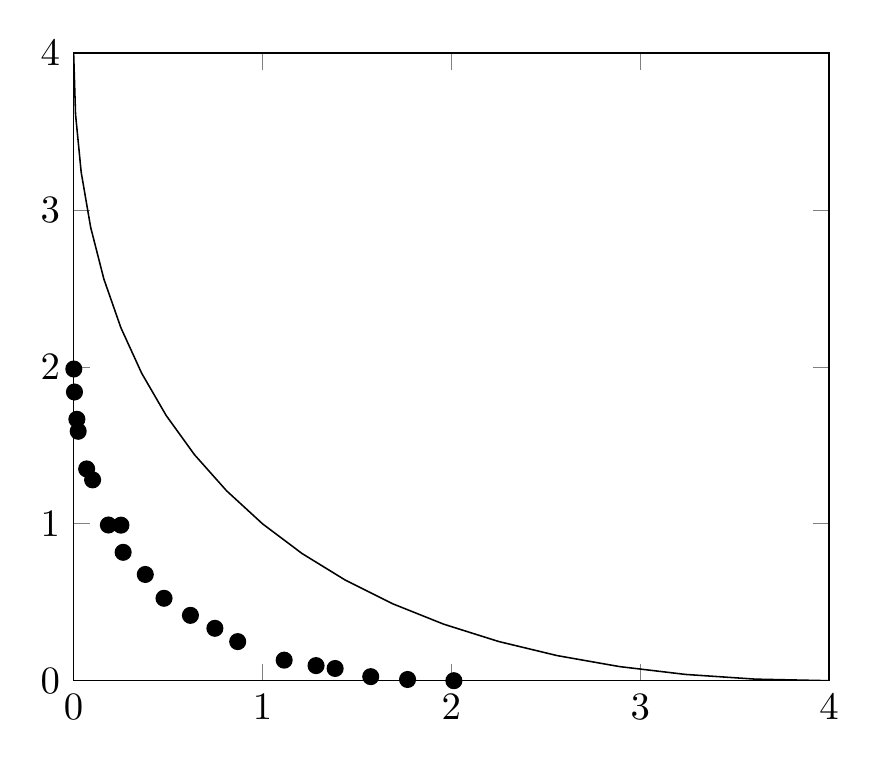
\begin{tikzpicture}[scale=1.4]
        \begin{axis}[enlargelimits=false]
            \addplot [] coordinates {
                (0.000000,4.000000) (0.010000,3.610000) (0.040000,3.240000) (0.090000,2.890000) (0.160000,2.560000) (0.250000,2.250000) (0.360000,1.960000) (0.490000,1.690000) (0.640000,1.440000) (0.810000,1.210000) (1.000000,1.000000) (1.210000,0.810000) (1.440000,0.640000) (1.690000,0.490000) (1.960000,0.360000) (2.250000,0.250000) (2.560000,0.160000) (2.890000,0.090000) (3.240000,0.040000) (3.610000,0.010000) (4.000000,0.000000) 
            };
            
            \addplot [only marks] coordinates {
                (2.013170,0.000022)(0.000811,1.986390)(1.114710,0.131126)(0.379304,0.677108)(0.478528,0.525250)(0.100382,1.280112)(1.767965,0.007815)(1.572890,0.025887)(0.262084,0.818221)(0.183932,0.992356)(0.868628,0.249256)(0.068938,1.349704)(0.024135,1.589631)(1.384435,0.078019)(0.004371,1.839921)(1.283436,0.096246)(0.618352,0.416527)(0.747836,0.333917)(0.017118,1.666182)(0.250461,0.991359) 
            };
        \end{axis}
    \end{tikzpicture}
\end{figure}
    \hrulefill

\end{document}
